\chapter{スケール、弦、そして26次元}

\lectureoverview{弦スペクトルの間隔を決めるものは何か。その答えは張力であり、質量の二乗の次元をもつ量である。基本弦について、この観察はプランク単位、直接励起の実際上の不可能性、そして強い重力の出現へと導く。意図的な中断の後、ボソン的開弦の基底状態に戻る。その零点エネルギーを正則化すると、歴史的な\emph{容易な}経路によって二十四個の横方向、したがって二十六個の時空次元が得られる。}

\section{我々が省いていたスケール}

これまで我々は、励起の1単位が何を意味するかを述べることなく、振動し回転する弦について語ってきた。ハドロンは弦として描くことができ、その振動子は励起されうるが、ある状態から次の状態への跳びはどれほど大きいのか。何がそれを決めるのか。

素弦模型には次元をもつパラメータがただ1つある。それを見出すには、普通の引き伸ばされたばねから始めればよい。その端点が\(\ell\)だけ離れているなら、フックの法則は次を与える。
\begin{equation}
  E_{\mathrm{spring}}=\frac{k\ell^2}{2}.
  \label{eq:l05-hooke}
\end{equation}
1/2の因子は、最初の版が書かれた後にクラスから提供された。この最初の見積もりでは、本質的なことは何もそのような数値因子に依存しない。

\begin{figure}[H]
  \centering
  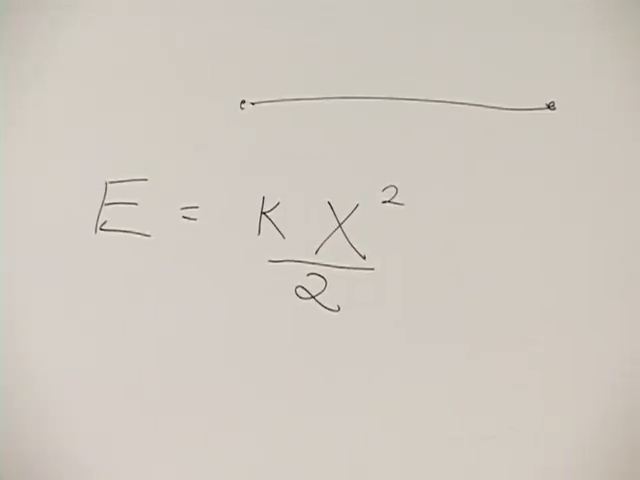
\includegraphics[width=0.72\textwidth]{lecture_05_figure_01.png}
  \caption{引き伸ばされた線分とそのフックの法則によるポテンシャルエネルギー。}
  \lectureframe{00:02:28}
  \label{fig:l05-hooke-board}
\end{figure}

\eqref{eq:l05-hooke}のエネルギーは非相対論的である。前の講義で用いた無限運動量の記述では、内部の非相対論的エネルギーは\(m\)ではなく\(m^2\)に比例する。したがって我々は模式的には次のように書く。
\begin{equation}
  m^2\sim k\ell^2,
  \qquad
  m\sim \sqrt{k}\,\ell.
  \label{eq:l05-mass-length}
\end{equation}
弦の静止系ではその質量はそのエネルギーであるから、第2の関係は次の形をとる。
\begin{equation}
  E_{\mathrm{rest}}\sim T_s\ell,
  \qquad
  T_s\equiv\sqrt{k}.
  \label{eq:l05-tension}
\end{equation}
係数\(T_s\)は弦の張力である。すなわち単位長さあたりに蓄えられるエネルギーである。

\begin{figure}[H]
  \centering
  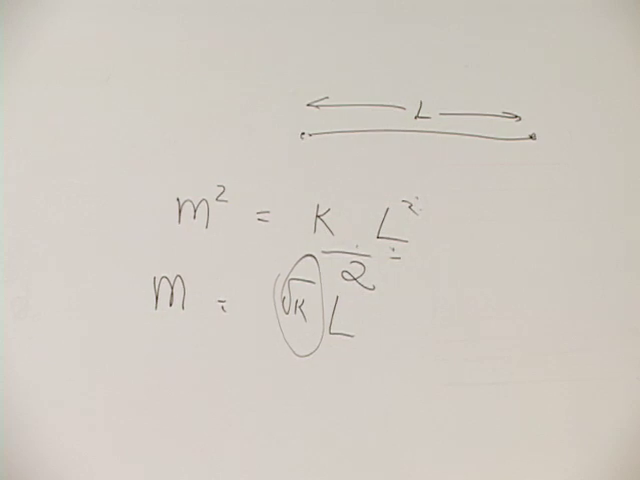
\includegraphics[width=0.78\textwidth]{lecture_05_figure_02.png}
  \caption{黒板は\(m^2\sim k\ell^2\)から長さに比例する質量へと移る。}
  \lectureframe{00:05:42}
  \label{fig:l05-mass-length-board}
\end{figure}

この記法は講義のばねの類推に合わせたものである。標準的な相対論的弦の記法では通常
\begin{equation}
  T_s=\frac{1}{2\pi\alpha'},
  \label{eq:l05-alpha-prime}
\end{equation}
と書くので、弦の準位の増分は\(m^2\)の増分を生み、それは\(1/\alpha'\)の程度、等価的に張力の程度である。
\editorialnote{講義における有効な\(k\)は、\(\sqrt{k}\)が張力の役割を果たすように選ばれている。規約に依存しない主張は、\(T_s\)が質量の二乗の次元をもち、レッジェ傾きが\(\alpha'\propto T_s^{-1}\)を満たすということである。}

\subsection{次元と振動子の間隔}

\(c=\hbar=1\)と置く。このときエネルギーは長さの逆数の次元をもつ：
\begin{equation}
  [E]=L^{-1}.
\end{equation}
張力は単位長さあたりのエネルギーであるから、
\begin{equation}
  [T_s]=L^{-2}=E^2.
  \label{eq:l05-tension-dimension}
\end{equation}
これが、弦スペクトルが自然に質量の二乗で間隔をなす理由である。

\begin{figure}[H]
  \centering
  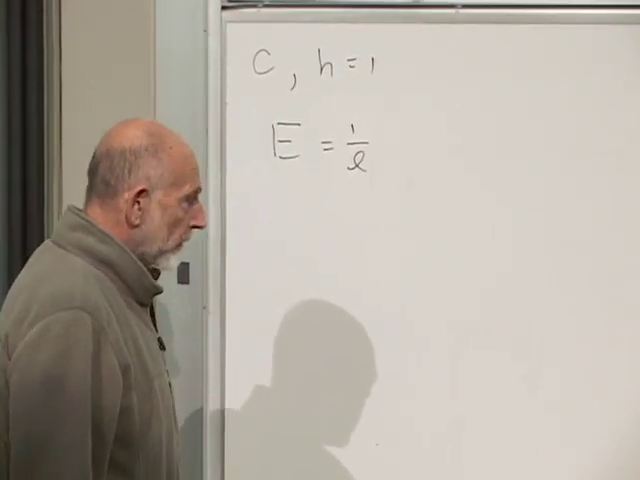
\includegraphics[width=0.68\textwidth]{lecture_05_figure_03.png}
  \caption{黒板上の自然単位: \(c=\hbar=1\)、エネルギーは長さの逆数であり、振動子の振動数はばねのスケールによって制御される。}
  \lectureframe{00:06:05}
  \label{fig:l05-natural-units-board}
\end{figure}

普通の振動子は別の方向から同じ点を明らかにする。質量\(\mu\)のばねに対して、
\begin{equation}
  \omega=\sqrt{\frac{k}{\mu}},
  \qquad
  \Delta E=\hbar\omega.
\end{equation}
より硬いばねはより高い振動数とより大きな量子間隔をもつ。弦はそのような基準モードを無限に含むが、それらの共通のスケールは\(T_s\)によって固定される。張力がわかれば、弦のスペクトルの間隔がわかる。

張力は力の次元ももつ。なぜなら力かける距離はエネルギーだからである。一方の端点を固定し、もう一方からおもりを吊るすことを想像しよう。\(E=T_s\ell\)である理想的な相対論的弦は、その長さに依存せず\(T_s\)によって定まる力を支えることができる。観測された励起エネルギーから推測されるハドロンの張力は、この意図的に空想的な比較では、トラックの重さに相当する。メソンからトラックが吊るされたことは一度もない。測定されたスペクトルが張力を与え、張力が力学的な比較を与えるのである。

基本弦ははるかに硬いであろう。それらが電子、光子、重力子の根底にあるなら、その最初の振動子励起は観測される粒子エネルギーのはるか上になければならない。同じ空想的な重力実験では、その張力は銀河程度の質量を支えうる。この比較の要点は工学ではない。巨大な張力は、大きな励起エネルギーと非常に小さな基底状態の揺らぎの両方を意味するということである。

\section{普遍定数から作られる単位}

どれほど巨大なスケールなら十分なのか。自然な基準はプランクスケールである。それを引用するのではなく、構成してみよう。

メートル、キログラム、秒は実験室単位として優れているが、その起源は人間の尺度にある。メートルは布やロープに便利であり、フィートは身体の一部にちなんで名付けられ、秒は1日の扱いやすい端数である。陽子半径を1に等しく置けばいくつかの核物理の公式は簡単になるかもしれないが、陽子は一つの特定の複合粒子にすぎない。そのような選択は物理学全体を簡単にはしない。

3つの次元定数はより普遍的な射程をもつ：
\begin{itemize}
  \item \(c\) はあらゆる物質系の限界速度を定め、
  \item \(\hbar\) はあらゆる量子系の不確定性関係に現れ、
  \item \(G\) は重力をあらゆる形の質量エネルギーに結びつける。
\end{itemize}
\(c=\hbar=G=1\) となる単位を選ぶことは、これらの定数から長さ、時間、質量の単位を構成することに等しい。

それらの通常の次元は
\begin{equation}
  \begin{aligned}
    [c]&=LT^{-1},
    & [\hbar]&=ML^2T^{-1},\\
    [G]&=L^3M^{-1}T^{-2}.
  \end{aligned}
  \label{eq:l05-dimensions-constants}
\end{equation}
である。中央の関係は
\(\Delta x\,\Delta p\gtrsim\hbar\)
から直接従う。最後の関係は、たとえば
\begin{equation}
  a=\frac{GM}{r^2}.
\end{equation}
から従う。

\begin{figure}[H]
  \centering
  \begin{minipage}[t]{0.48\textwidth}
    \centering
    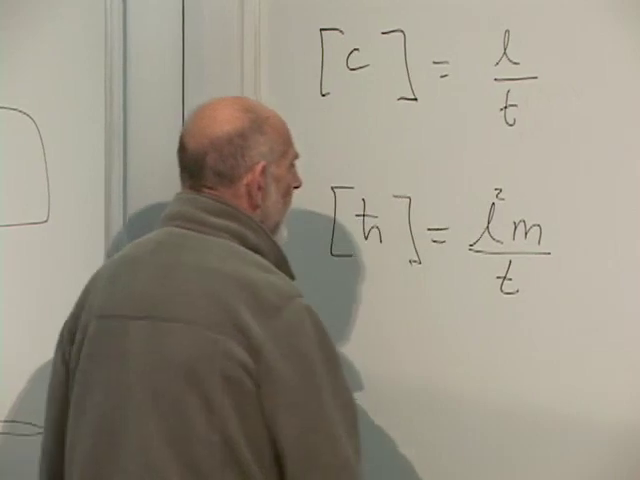
\includegraphics[width=\textwidth]{lecture_05_figure_04.png}
    \par\smallskip\footnotesize (a) \(c\) と \(\hbar\) の単位。
  \end{minipage}\hfill
  \begin{minipage}[t]{0.48\textwidth}
    \centering
    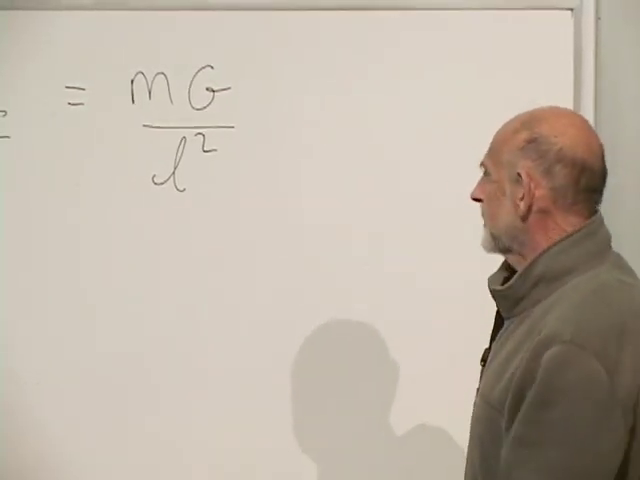
\includegraphics[width=\textwidth]{lecture_05_figure_05.png}
    \par\smallskip\footnotesize (b) ニュートン加速度による \(G\) の単位。
  \end{minipage}
  \caption{授業で組み立てられた次元解析の材料。}
  \lectureframe{00:25:43--00:26:40}
  \label{fig:l05-dimensional-analysis-board}
\end{figure}

\subsection{まずプランク面積}

次元が \(L^2\) となるような冪 \(p,q,r\) を求める：
\begin{equation}
  G^p\hbar^q c^r
\end{equation}
面積を最初に選ぶことで早い段階での平方根を避けられ、また後に重力において面積が果たす特別な役割を先取りすることにもなる。
\eqref{eq:l05-dimensions-constants} から、質量と時間の消去により
\begin{equation}
  -p+q=0,
  \qquad
  -2p-q-r=0.
\end{equation}
が得られる。残る長さの冪は
\begin{equation}
  3p+2q+r=2.
\end{equation}
を満たさなければならない。したがって \(q=p\)、\(r=-3p\)、\(p=1\) である。プランク面積は
\begin{equation}
  \ell_P^2=\frac{G\hbar}{c^3},
  \label{eq:l05-planck-area}
\end{equation}
であり、その結果
\begin{equation}
  \ell_P=\sqrt{\frac{G\hbar}{c^3}},
  \qquad
  t_P=\frac{\ell_P}{c},
  \qquad
  m_P=\sqrt{\frac{\hbar c}{G}}.
  \label{eq:l05-planck-units}
\end{equation}

\begin{figure}[H]
  \centering
  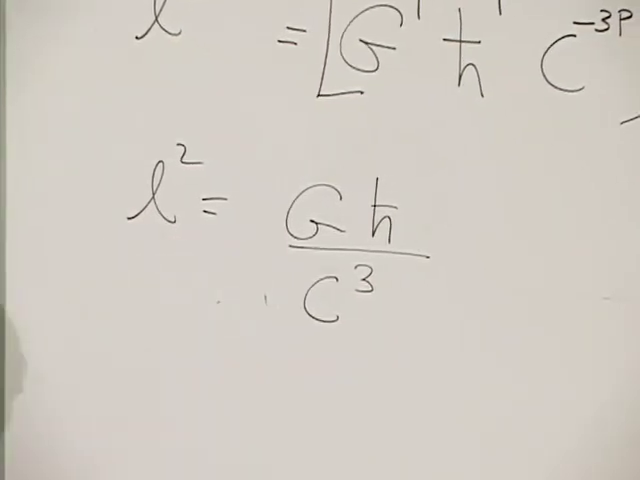
\includegraphics[width=0.78\textwidth]{lecture_05_figure_06.png}
  \caption{プランク面積と長さについての完成した次元論的議論。}
  \lectureframe{00:31:34}
  \label{fig:l05-planck-area-board}
\end{figure}

桁程度の精度では、
\begin{equation}
  \begin{aligned}
    \ell_P&\sim10^{-35}\,\mathrm{m},
    &t_P&\sim10^{-43}\,\mathrm{s},\\
    m_P&\sim10^{-8}\,\mathrm{kg},
    &m_Pc^2&\sim10^{19}\,\mathrm{GeV}.
  \end{aligned}
  \label{eq:l05-planck-numbers}
\end{equation}

\begin{figure}[H]
  \centering
  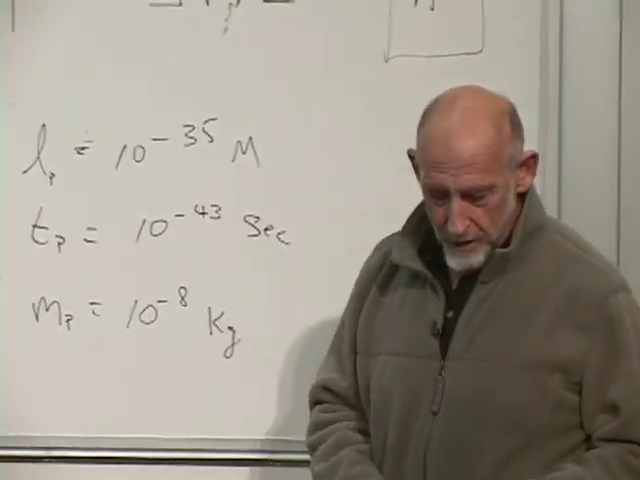
\includegraphics[width=0.72\textwidth]{lecture_05_figure_07.png}
  \caption{桁程度まで記録された3つのプランクスケール。}
  \lectureframe{00:35:12}
  \label{fig:l05-planck-values-board}
\end{figure}

その長さと時間は想像を絶するほど小さいが、質量は素粒子の基準からすれば驚くほど巨視的であり、およそ細かい塵の粒ほどの質量である。その静止エネルギーは数ギガジュールの程度で、ガソリンタンク一杯分の化学エネルギーに匹敵する。これに対して観測可能な宇宙は、およそ\(10^{60}\)プランク長にわたり、およそ\(10^{60}\)プランク時間のあいだ存在してきた。これらの比較は、単位に物理的な重みを与えるためのものであり、その数値精度を高めるためのものではない。

特性弦長 \(\ell_s=\sqrt{\alpha'}\) が \(\ell_P\) の近くにあれば、弦の量子的な大きさは \(\ell_P\) の近くにあり、その振動周期は \(t_P\) の近くにあり、その最初の質量励起は \(m_P\) の近くにある。講義は10倍、100倍、あるいはそれ以上の因子を許容している。この同一視は期待であって、次元的な恒等式ではない。

\begin{classroomqa}
\audiencequestion{プランクスケールの質量とは、粒子の基底状態からの増加分のことですか？ \lecturetimestamp{00:38:37}}
\lecturerresponse{等間隔に並ぶ量は質量の二乗である。基底状態が軽いなら、第一の弦励起状態は\(m^2\)が\(m_P^2\)程度だけ大きくなり、したがってその質量と必要な重心系エネルギーは\(m_P\)程度となる。}
\end{classroomqa}

\section{2つのスケールはどれほど近いべきか？}

\begin{classroomqa}
\audiencequestion{次元解析は \(\ell_P\) を与えるが、なぜその数が弦の長さでなければならないのか？\lecturetimestamp{00:40:21}}
\lecturerresponse{それは重力によって、また観測される弦構造の不在によって支持される物理的な推測であり、次元解析だけから従う帰結ではない。弦長はプランク長より大きくてもよく、その場合そのエネルギー尺度はより低い。講義が主張するのは、それが通常の素粒子物理の長さであってはならないということ、そしてそれをプランク長よりはるかに下に押しやると重力崩壊に突き当たるということだけである。}
\end{classroomqa}

2つのスケールの関係は実際には結合定数に依存する。完全なコンパクト化では、\(\ell_P\)、\(\ell_s\)、弦結合定数、およびコンパクト化体積が一緒に関与する。普遍的な方程式 \(\ell_s=\ell_P\) は存在しない。講義から残るのはスケールに関する議論である：弦の効果は非常に高いところで現れなければならず、プランク以下の局在化は重力を無視して論じることはできない。
\editorialnote{現代の弦の構成は、弦長を4次元プランク長と正確に同一視する必要はない。それらの関係は弦結合定数とコンパクト化のデータに依存する。}

\begin{classroomqa}
\audiencequestion{プランク長を最小の有用な長さとみなすなら、プランク質量も可能な最小の質量なのでしょうか。\lecturetimestamp{00:43:27}}
\lecturerresponse{いいえ。通常の粒子はずっと軽いです。プランク質量は、コンパクトな物体がその量子波長に匹敵する重力半径を持ちうるスケールです。講義のヒューリスティックな言葉で言えば、それは最も軽い半古典的ブラックホールのスケールであり、その寿命はプランク時間の程度です。最後の記述は、完全に量子的な物体の正確な記述と誤解されるべきではありません。}
\end{classroomqa}

\subsection{走る結合定数が教えてくれること}

従来の量子場理論が、加速器の直接到達範囲をはるかに超えるスケールまで有効であり続けるという間接的な証拠がある。3つの標準模型ゲージ結合定数は到達可能なエネルギーで測定され、そのスケール依存性は外挿できる。講義の模式的なプロットでは、\(U(1)\)、\(SU(2)\)、\(SU(3)\)の結合定数が高い大統一スケール、おそらくプランクエネルギーの数桁下で互いに近づく。

\begin{figure}[H]
  \centering
  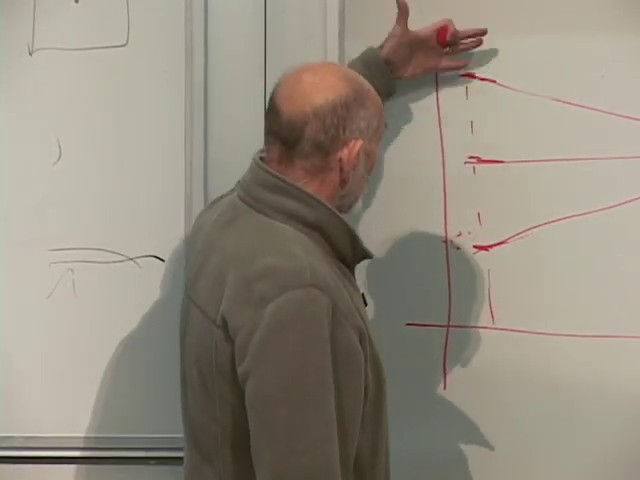
\includegraphics[width=0.70\textwidth]{lecture_05_figure_08.png}
  \caption{模式的な走る結合定数のプロット。3つのゲージ曲線は、増大する重力の強さが1程度になる前に互いに近づく。}
  \lectureframe{00:47:18}
  \label{fig:l05-running-couplings-board}
\end{figure}

これは外挿であり、交差点での直接実験ではない。実験室と大統一エネルギーの間の追加粒子や閾値は傾きを変えうる。慎重な結論は、既知の場の理論が通常の距離で弦サイズの下部構造の兆候を示さないこと、そしてもっともらしい弦スケールが推論された大統一スケールとプランクスケールの間の巨大な間隔のどこかにあることだけである。

\begin{classroomqa}
\audiencequestion{どの3つの結合定数が外挿されているのですか。\lecturetimestamp{00:48:28}}
\lecturerresponse{それらは\(U(1)\)、\(SU(2)\)、\(SU(3)\)に関連するゲージ結合定数である。すなわち超電荷、弱い相互作用、強い相互作用である。電磁気学はこの計算では独立した第4のゲージ因子ではなく、電弱混合から現れる。}
\end{classroomqa}

\begin{classroomqa}
\audiencequestion{重力定数\(G\)自体は、より高いエネルギーを探るにつれて増大するのですか。\lecturetimestamp{00:49:30}}
\lecturerresponse{\(G\)は次元を持つので、それ自体は無次元のゲージ結合定数と比較するのに正しい量ではない。特性エネルギー\(M\)では、無次元の重力の強さは模式的に\(GM^2/(\hbar c)\)のように振る舞う。その組み合わせはエネルギーとともに増大し、プランクスケールで1程度になる。}
\end{classroomqa}

力の法則が比較を可視化する：
\begin{equation}
  F_{\mathrm{em}}\sim\frac{e^2}{r^2},
  \qquad
  F_{\mathrm{grav}}\sim\frac{GM^2}{r^2}.
  \label{eq:l05-force-laws}
\end{equation}
したがって\(e^2\)は\(G\)と比較されるのではなく、自然単位で\(GM^2\)と比較される。

\begin{figure}[H]
  \centering
  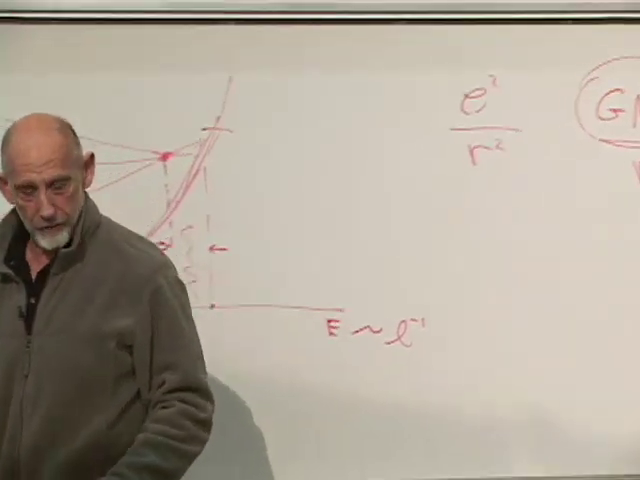
\includegraphics[width=0.74\textwidth]{lecture_05_figure_09.png}
  \caption{無次元の重力の強さを特定するために用いられる電磁気力と重力の法則。}
  \lectureframe{00:50:50}
  \label{fig:l05-force-laws-board}
\end{figure}

\section{直接弦分光が遠い理由}

電子が弦であることを実験的にどうやって確立するだろうか。ハドロン分光が行ったことをするだろう。すなわち、内部モードを励起するのに十分強く叩き、質量が弦のパターンに従うタワーを探すのである。最初の質量を持つ準位が\(10^{19}\,\mathrm{GeV}\)付近にあるなら、それはどんな直接機械をもはるかに超えている。

全エネルギーだけが障害ではない。それは微小な衝突パラメータ内に集中されなければならない。そこにブラックホールが関わってくる。

\begin{classroomqa}
\audiencequestion{これらのエネルギーで加速器は小さなブラックホールを生成し始めるでしょうか。\lecturetimestamp{00:50:57}}
\lecturerresponse{重心エネルギーがその重力半径内に集中されれば、それがヒューリスティックな期待である。恒星ブラックホールは重力ポテンシャルエネルギーが大質量星を圧縮することで作られる。微視的なものは代わりに、微小な衝突領域に集束された運動エネルギーによって作られるだろう。4次元重力では、必要なスケールはプランク的である。}
\end{classroomqa}

参考までに、線形加速器のエネルギー利得はほぼその長さに比例する。講義では、単純なSLAC規模の尺度として約2マイルでおよそ\(100\,\mathrm{GeV}\)を取る。同じ勾配で\(10^{19}\,\mathrm{GeV}\)に到達するには、長さをおよそ\(10^{17}\)倍にし、銀河規模の機械を生み出すことになる。

そのような機械でも光度が必要である。ビームはプランク長の精度で一度に一対ずつ狙われるのではない。膨大な数の粒子が交差し、少数が所望の衝突パラメータで衝突する。プランクエネルギーに膨大な衝突率を掛けると、同様に不合理な電力要件が生じる。推定は意図的に粗いが、その結論は安定している。プランクスケールでの直接弦分光は、もっともらしく設計できる実験ではない。

間接的な証拠は、より構造的なものでなければならないだろう。すなわち、観測されている低エネルギー粒子と相互作用を、検証に足るだけの具体性をもって導き出す理論か、弦スケールよりはるかに低いところまで生き残るコンパクト化の効果である。この講義は、そのような決定的な構成がすでに手に入っていると主張しているわけではない。

\subsection{余剰次元と局在化の限界}

\begin{classroomqa}
\audiencequestion{余剰次元もまたプランク長に近い大きさをもつべきなのだろうか。\lecturetimestamp{00:56:23}}
\lecturerresponse{この初等的な描像では、それらは極端に小さいと期待されるが、その議論によって厳密に固定されるわけではない。もしコンパクトな次元が、より低いエネルギーで探れるほど大きければ、新しいKaluza--Kleinモードと高次元の振る舞いが、すでに我々の観測する場の理論を変えてしまっているはずである。したがって、その成功した外挿は、そうした次元に上限を与える。}
\end{classroomqa}

\begin{classroomqa}
\audiencequestion{なぜ弦やコンパクト次元は\(\ell_P\)より何桁も小さくなりえないのか。\lecturetimestamp{00:57:48}}
\lecturerresponse{より短い距離を分解するには、より大きな運動量が必要である。プランクスケールを超えると、局在化に必要なエネルギーは、探っている領域と同程度の、そしてやがてそれより大きな重力半径をもつ。実験は、より小さな通常の弦を分解する前に、ブラックホールを作ってしまうのである。}
\end{classroomqa}

不確定性原理がその見積もりを与える。\(\Delta x\)に局在化するには、次が必要である。

\begin{classroomqa}
\audiencequestion{プランク長とプランク時間が選ばれたとき、プランク質量は物理的にどのように決まるのか。\lecturetimestamp{00:59:04}}
\lecturerresponse{\(\hbar\)または\(G\)のいずれかを用いて、長さのスケールをエネルギーに変換する。不確定性原理によれば、二つの粒子を\(\ell_P\)以内に局在化するには\(\hbar/\ell_P\)程度の運動量、したがって\(m_Pc^2\)程度のエネルギーが必要である。等価に言えば、それは量子長と重力長が同程度になる質量である。}
\end{classroomqa}

\begin{equation}
  \Delta p\gtrsim\frac{\hbar}{\Delta x},
  \qquad
  E\sim c\,\Delta p.
  \label{eq:l05-localization}
\end{equation}
\(\Delta x=\ell_P\)において、このエネルギーは
\begin{equation}
  E\sim\frac{\hbar c}{\ell_P}=m_Pc^2.
\end{equation}
である。同時にシュヴァルツシルト半径
\begin{equation}
  r_s\sim\frac{GE}{c^4}
\end{equation}
は、数値定数を除いて\(\ell_P\)程度である。量子局在化と重力崩壊は同じスケールで出会う。

\begin{figure}[H]
  \centering
  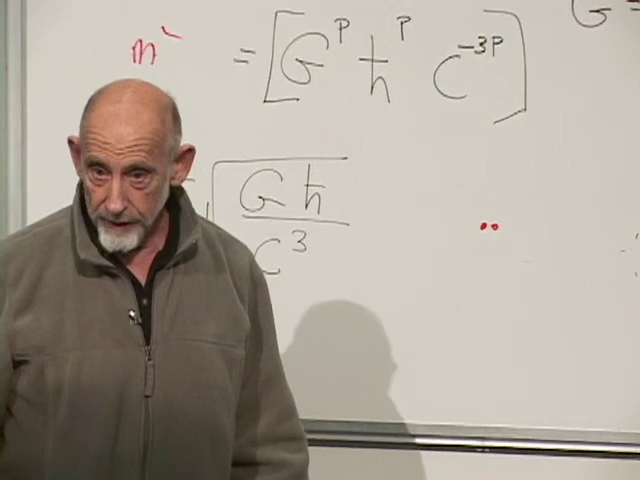
\includegraphics[width=0.74\textwidth]{lecture_05_figure_10.png}
  \caption{局在化の議論の間に再訪されたプランク長と質量の公式。}
  \lectureframe{01:00:25}
  \label{fig:l05-localization-board}
\end{figure}

これでスケール設定の議論が完了する。

\section{基底状態は光子より下に位置しなければならない}

休憩の後には二つの可能な方向がある。共形変換を始めるか、臨界次元へのより古く容易な道を与えるかである。我々は後者を選ぶが、一つ警告しておく。容易な議論は容易ではなく、最も深い理由でもない。それでもなおそれは正しく、歴史的発見に近いものである。

開いたボソン弦に戻ろう。横方向の生成演算子を一度作用させると、二つの偏極状態が生じる。縦方向の第三の状態が存在しないため、この励起は質量ゼロのベクトルでなければならない。1モード\(1\)の量子が\(m^2\)を1だけ上げる単位では、
\begin{equation}
  m_{\mathrm{ground}}^2=-1,
  \qquad
  m_{\mathrm{first}}^2=-1+1=0.
  \label{eq:l05-open-intercept}
\end{equation}
タキオン的基底状態はボソン理論の問題として残る。それは認められ、脇に置かれる。当面の問いは、\eqref{eq:l05-open-intercept}における負の単位がどこから来るのかである。

すべての弦モードは調和振動子である。\(\hbar=1\)のもとで、その真空エネルギーは
\begin{equation}
  E_{0,n}=\frac{\omega_n}{2}.
\end{equation}
である。弦の場合、\(\omega_n=n\)なので、一つの横方向座標は形式的に
\begin{equation}
  E_0^{(1)}
  =\frac12\sum_{n=1}^{\infty}n.
  \label{eq:l05-formal-zero-point}
\end{equation}
を寄与する。

\begin{figure}[H]
  \centering
  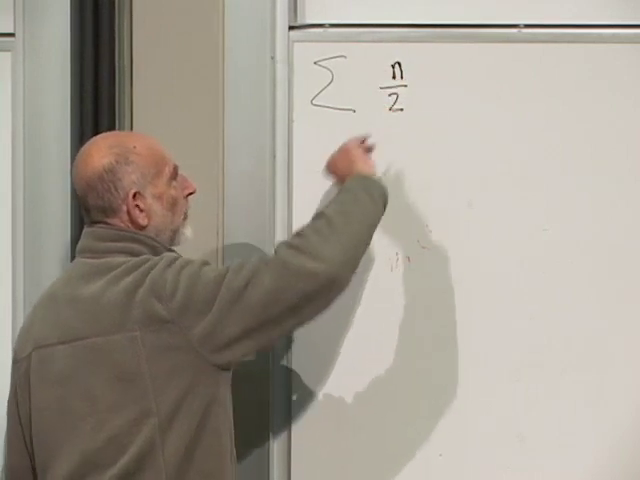
\includegraphics[width=0.70\textwidth]{lecture_05_figure_11.png}
  \caption{モード振動数が思い出された後に書かれた零点和\(\sum n/2\)。}
  \lectureframe{01:06:18}
  \label{fig:l05-zero-point-board}
\end{figure}

ここで困難は鋭くなる。
\eqref{eq:l05-formal-zero-point}の各項は正であり、和は発散する。どのようにしてそれが有限な負の切片を与えうるのか。

\section{スペクトルを読む前に運動を差し引く}

和を正則化する前に、なぜ内部エネルギーが質量の二乗と同一視されたのかを思い出そう。大きな縦方向運動量\(P>0\)をもつ粒子に対して、
\begin{equation}
  E=\sqrt{P^2+m^2}
   =P+\frac{m^2}{2P}
   +O(P^{-3}).
  \label{eq:l05-large-p-energy}
\end{equation}

\begin{figure}[H]
  \centering
  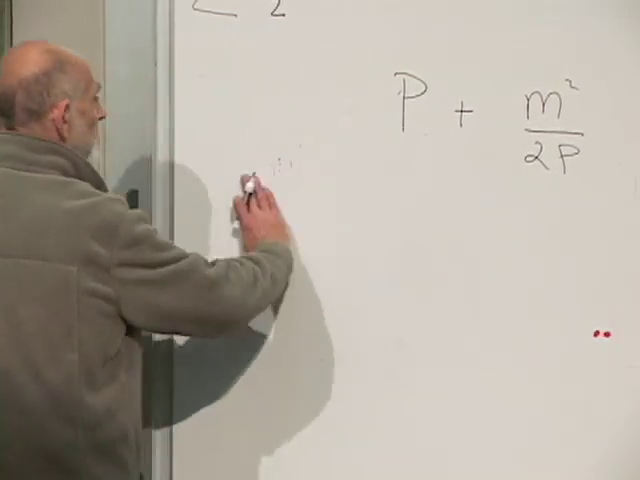
\includegraphics[width=0.70\textwidth]{lecture_05_figure_12.png}
  \caption{全体の運動量を内部質量項から分離する大きな\(P\)での展開。}
  \lectureframe{01:07:35}
  \label{fig:l05-fast-energy-board}
\end{figure}

第一項は\(z\)軸に沿った、興味のない全体の運動である。それは保存され、同じ\(P\)をもつすべての内部状態に共通である。それを差し引き、再スケールすると、運動学的な時間の遅れが取り除かれる。
\begin{equation}
  \begin{aligned}
    E-P&=\frac{m^2}{2P}+O(P^{-3}),\\
    2P(E-P)&=m^2+O(P^{-2}).
  \end{aligned}
  \label{eq:l05-internal-energy}
\end{equation}

原子が物理的な描像を与える。水素原子をブーストしよう。その全エネルギーは増大するが、実験室時間で測った二つの内部準位間のエネルギー差は、原子の時計が遅れるために縮む。\eqref{eq:l05-large-p-energy}における因子\(1/P\)がその抑制である。\(2P\)を掛けると、不変な質量の二乗の差が回復する。

したがって、生の基底状態エネルギーは文字通り\(-1\)である必要はない。それは全体的な縦方向エネルギーに伴う大きな状態に依存しない部分と、有限な内部の残りを含んでいてもよい。講義では、振動子の和に戻る前に、両方の部分を表示するためにブーストされた関係を書き直す。

\begin{figure}[H]
  \centering
  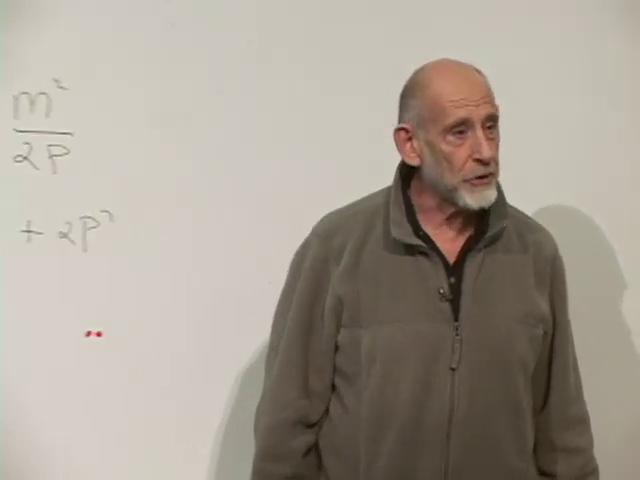
\includegraphics[width=0.76\textwidth]{lecture_05_figure_13.png}
  \caption{大きな状態に依存しない縦方向の寄与の隣に表示された不変質量項。}
  \lectureframe{01:11:34}
  \label{fig:l05-infinite-piece-board}
\end{figure}

無限の真空エネルギーは量子場の理論でよく知られている。しばしば、発散する状態に依存しない定数を観測可能なエネルギー差から分離する。講義ではこれを部屋の中の電磁場の零点エネルギーと比較し、この手続きを不満足ではあるが標準的であると率直に呼んでいる。ここでは同じヒューリスティックに従う。すなわち、発散部分を分離し、確定した有限の残りが生き残るかどうかを問う。

\section{和の正則化}

正の正則化子\(\epsilon\)を導入する：
\begin{equation}
  S_1(\epsilon)
  =\sum_{n=1}^{\infty}n e^{-n\epsilon}.
  \label{eq:l05-regulated-sum}
\end{equation}
すべての\(\epsilon>0\)に対して、指数関数は最終的に因子\(n\)を打ち負かすので、和は収束する。\(\epsilon\)をゼロに近づけるとカットオフが取り除かれる。

\begin{figure}[H]
  \centering
  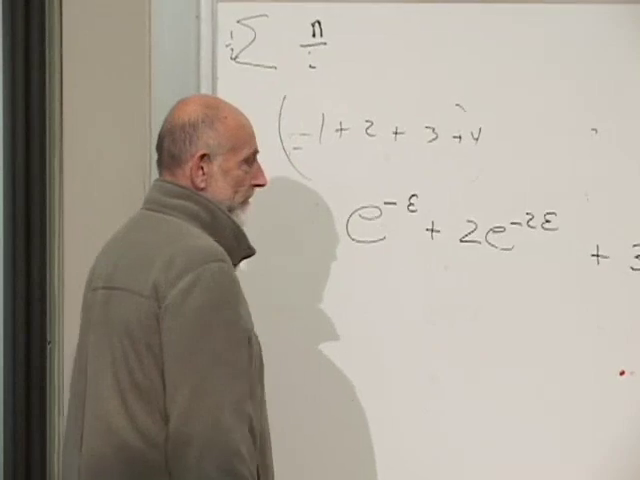
\includegraphics[width=0.78\textwidth]{lecture_05_figure_14.png}
  \caption{\(1+2+3+\cdots\)に項ごとに適用された指数関数的正則化子。}
  \lectureframe{01:16:42}
  \label{fig:l05-regulator-board}
\end{figure}

因子\(n\)は微分によって生成できる：
\begin{equation}
  S_1(\epsilon)
  =
  -\frac{d}{d\epsilon}
  \sum_{n=1}^{\infty}e^{-n\epsilon}.
  \label{eq:l05-derivative-trick}
\end{equation}

\begin{figure}[H]
  \centering
  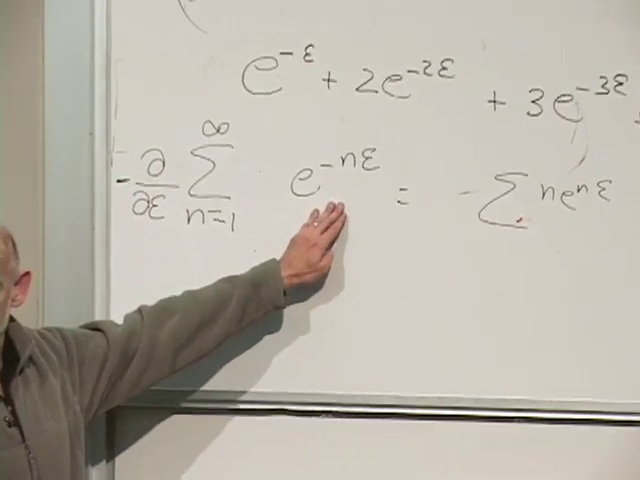
\includegraphics[width=0.76\textwidth]{lecture_05_figure_15.png}
  \caption{カットオフに関する微分が\(-n\)を引き下ろす。}
  \lectureframe{01:18:05}
  \label{fig:l05-derivative-board}
\end{figure}

残りの級数は幾何級数である：
\begin{equation}
  S_0(\epsilon)
  \equiv
  \sum_{n=1}^{\infty}e^{-n\epsilon}
  =
  \frac{e^{-\epsilon}}{1-e^{-\epsilon}}
  =
  \frac{1}{e^\epsilon-1}.
  \label{eq:l05-geometric-sum}
\end{equation}

\begin{figure}[H]
  \centering
  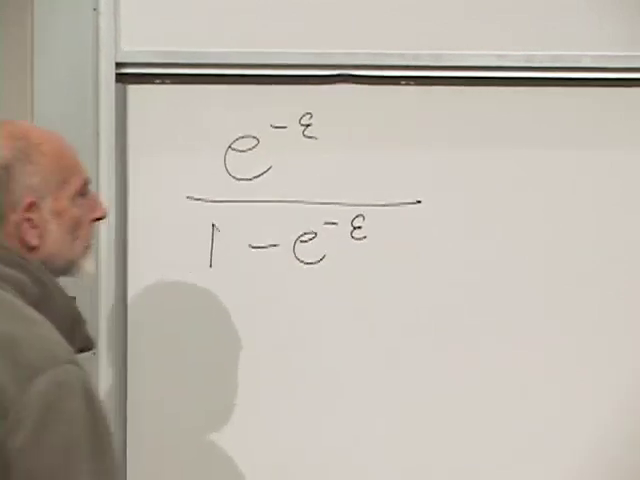
\includegraphics[width=0.68\textwidth]{lecture_05_figure_16.png}
  \caption{閉じた形での正則化された幾何級数。}
  \lectureframe{01:19:12}
  \label{fig:l05-geometric-board}
\end{figure}

小さい\(\epsilon\)で展開する：
\begin{equation}
  S_0(\epsilon)
  =
  \frac{1}{\epsilon}
  -\frac12
  +\frac{\epsilon}{12}
  -\frac{\epsilon^3}{720}
  +O(\epsilon^5).
  \label{eq:l05-bernoulli-expansion}
\end{equation}
黒板では、分子と分母を別々に展開し、\(\epsilon\)の1乗をくくり出し、次に逆数を展開することによってこれを得る。その計算には授業中のいくつかの符号の確認が含まれており、コンパクトな式\eqref{eq:l05-bernoulli-expansion}がその整理された結果である。

\begin{figure}[H]
  \centering
  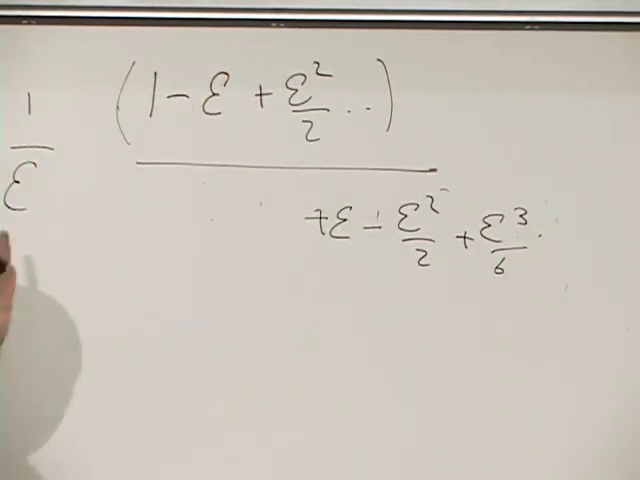
\includegraphics[width=0.78\textwidth]{lecture_05_figure_17.png}
  \caption{逆数が簡略化される前の分子と分母の展開。}
  \lectureframe{01:23:10}
  \label{fig:l05-expansion-board}
\end{figure}

\(-d/d\epsilon\)を適用すると次を得る：
\begin{equation}
  S_1(\epsilon)
  =
  \frac{1}{\epsilon^2}
  -\frac{1}{12}
  +\frac{\epsilon^2}{240}
  +O(\epsilon^4).
  \label{eq:l05-regulated-result}
\end{equation}

\begin{figure}[H]
  \centering
  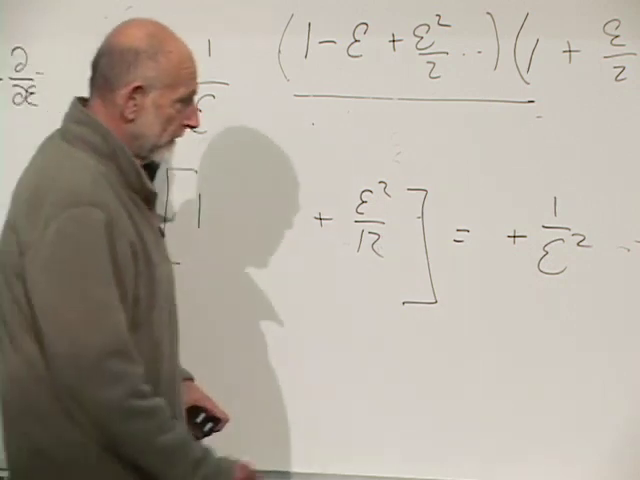
\includegraphics[width=0.78\textwidth]{lecture_05_figure_18.png}
  \caption{正則化子計算の最後における発散する\(1/\epsilon^2\)項と有限な\(-1/12\)の残り。}
  \lectureframe{01:29:48}
  \label{fig:l05-minus-twelve-board}
\end{figure}

この結果を冗談めかして\(1+2+3+\cdots=-1/12\)と要約するのはよくあることである。それは通常の収束ではない。式\eqref{eq:l05-regulated-result}は、この特定の正則化子が発散項と正則化子に依存しない有限部分を生み出すことを述べている：
\begin{equation}
  \underbrace{\frac{1}{\epsilon^2}}_{\text{divergent}}
  \;+\;
  \underbrace{\left(-\frac{1}{12}\right)}_{\text{finite}}
  \;+\;O(\epsilon^2).
\end{equation}
講義では第一項をすでに存在する状態に依存しない部分に吸収し、第二項を保持する。また、パウリに帰せられる警告も保持する。すなわち、無限であること自体は量をゼロにするものではない。一貫した理論は、なぜ引き算が許されるのかを説明しなければならない。

\eqref{eq:l05-formal-zero-point}における1/2の因子を復元すると、1つの横座標が寄与する：
\begin{equation}
  E_0^{(1)}=-\frac{1}{24}.
  \label{eq:l05-one-transverse-zero-point}
\end{equation}

\begin{figure}[H]
  \centering
  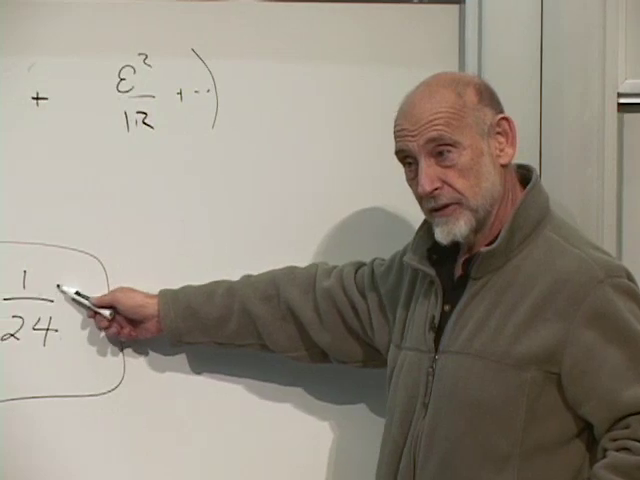
\includegraphics[width=0.68\textwidth]{lecture_05_figure_19.png}
  \caption{1/2の因子が有限な\(-1/12\)を横座標あたり\(-1/24\)に変換する。}
  \lectureframe{01:33:42}
  \label{fig:l05-minus-twenty-four-board}
\end{figure}

\section{横方向の数え上げ}

\(D_\perp\)を横方向の弦座標の数とする。それらの全真空寄与は
\begin{equation}
  E_0^{\mathrm{open}}
  =-\frac{D_\perp}{24}.
  \label{eq:l05-open-vacuum}
\end{equation}
最初の開弦振動子が基底状態を\(-1\)から質量ゼロの準位へ上げるためには、次が必要である：
\begin{equation}
  -\frac{D_\perp}{24}=-1.
\end{equation}
したがって
\begin{equation}
  D_\perp=24.
\end{equation}
これらは大きな縦方向運動量に垂直な方向である。その縦方向の空間方向と時間を加えると
\begin{equation}
  D=D_\perp+2=26.
  \label{eq:l05-critical-dimension}
\end{equation}

\begin{classroomqa}
\audiencequestion{この議論はいつ弦理論に入ったのか？\lecturetimestamp{01:35:27}}
\lecturerresponse{それは元のハドロン弦の時代、およそ1969年と1970年代初頭に属する。レッジェ軌跡はすでに実験的に知られていた。振動子模型がそれ自体として探究されると、第一励起状態は3つではなく2つのベクトル偏極を持つことがわかり、質量ゼロであることを強いられた。その結果必要とされる切片は、すぐに24個の横方向振動子へと導いた。}
\end{classroomqa}

当時、これは信じがたいほど奇妙に見えた。なぜ正則化された真空の和が時空の次元を知っているべきなのか？しかし、各部分は一致した。質量ゼロのベクトル、切片、横方向振動子の数はすべて同じ数を選び出した。

\subsection{閉弦が数え上げを確認する}

閉弦が最初の物理的な質量ゼロ準位に到達するには、1つの左巻きモードと1つの右巻きモードが必要である。したがってその基底状態はゼロより2単位下から始まらなければならない。

\begin{classroomqa}
\audiencequestion{24個の横方向が\(-1\)しか与えないなら、閉じた弦は48個の横方向に住まなければならないのか？\lecturetimestamp{01:37:47}}
\lecturerresponse{いいえ。同じ時空には開いた弦と閉じた弦の両方が存在する。閉じた弦はすでに2倍の振動子内容を持っている。すなわち、各世界面方向を循環する1つのタワーである。各タワーは\(-24/24=-1\)に寄与するので、合わせて\(-2\)を与える。}
\end{classroomqa}

したがって
\begin{equation}
  E_0^{\mathrm{closed}}
  =
  2\left(-\frac{D_\perp}{24}\right)
  =-2
  \qquad (D_\perp=24).
\end{equation}
各セクターから1つの振動子を加えると、状態は2単位だけ上がり、質量の二乗がゼロになる。これはまさに、前の講義でグラビトン多重項が現れた場所である。

この一致によって議論はより良く見えるが、それでも深い説明ではない。現代の量子化では、正規順序定数、ローレンツ代数またはビラソロ代数の閉包性、そして共形アノマリーの相殺は、1つの整合した構造に属する。その構造が切片と臨界次元の両方を固定する。有限なカットオフの残りは、そこへ至る歴史的な道筋である。
\editorialnote{調節計算は正規順序定数のヒューリスティックな見方である。\(D=26\)のより深い導出には、世界面の共形不変性、等価的に共形アノマリーの相殺と整合した拘束代数が必要である。}

そのより深い道筋が次に来る。始めるにはほんの少しの複素解析があればよい。複素座標、解析関数、そしてコーシー--リーマンの方程式である。約束された物理的イメージは、トルコのタフィー---を一方向に引っ張り、別の方向に伸ばし、重要な構造を壊すことなく形を変えることである。そのイメージの背後にある数学は共形不変性である。
